\documentclass[12pt, a4paper]{report}

\usepackage{amsmath,amsthm,amssymb}
\usepackage{mathtext}
\usepackage[T1,T2A]{fontenc}
\usepackage[utf8]{inputenc}
\usepackage[english,russian]{babel}
\usepackage{listings}
\usepackage{graphicx}
\usepackage{tablefootnote}
\usepackage{indentfirst}
\usepackage{color}
\usepackage{float}
\usepackage{caption}
\captionsetup[table]{singlelinecheck=off}
\captionsetup[lstlisting]{singlelinecheck=off, labelformat=empty}
\usepackage{pgfplots}
\pgfplotsset{compat=1.9}
\usepackage[left=3cm,right=1cm, top=2cm,bottom=2cm,bindingoffset=0cm]{geometry}
\graphicspath{{./img/}}

% Настройка заголовков
\makeatletter
\renewcommand\LARGE{\@setfontsize\LARGE{20pt}{30}}
\renewcommand\Large{\@setfontsize\Large{16pt}{20}}
\renewcommand\large{\@setfontsize\large{14pt}{20}}
\makeatother
\RequirePackage{titlesec}
\titleformat{\chapter}{\LARGE\bfseries}{\thechapter}{14pt}{\LARGE\bfseries}
\titleformat{\section}{\Large\bfseries}{\thesection}{14pt}{\Large\bfseries}
\titleformat{\sub}{\large\bfseries}{\thesubsection}{14pt}{\large\bfseries}
\titlespacing{\chapter}{12.5mm}{-35pt}{40pt}
\titlespacing{\section}{12.5mm}{20pt}{20pt}
\titlespacing{\subsection}{12.5mm}{10pt}{10pt}

\lstset{ 
	backgroundcolor=\color{white},   % choose the background color; you must add \usepackage{color} or \usepackage{xcolor}; should come as last argument
	breaklines=true,                 % sets automatic line breaking
	captionpos=t,                    % sets the caption-position to bottom
	commentstyle=\color{green},    % comment style
	keywordstyle=\color{blue},       % keyword style
	language=Python,                 % the language of the code
	numbers=left,                    % where to put the line-numbers; possible values are (none, left, right)
	numbersep=5pt,                   % how far the line-numbers are from the code
	numberstyle=\tiny\color{black}, % the style that is used for the line-numbers
	showspaces=false,                % show spaces everywhere adding particular underscores; it overrides 'showstringspaces'
	showstringspaces=false,          % underline spaces within strings only
	showtabs=false,                  % show tabs within strings adding particular underscores
	stepnumber=1,                    % the step between two line-numbers. If it's 1, each line will be numbered
	stringstyle=\color{yellow},     % string literal style
	tabsize=2,	                   % sets default tabsize to 2 spaces
	frame=single
}

\begin{document}
	
	\begin{titlepage}
		\noindent \begin{minipage}{0.15\textwidth}
			
\includegraphics[width=\linewidth]{bauman_image.jpg}
		\end{minipage}
		\footnotesize\noindent \begin{minipage}{0.8\textwidth}\centering
			\textbf{Министерство науки и высшего образования Российской Федерации}\\
			\textbf{Федеральное государственное бюджетное образовательное учреждение}\\
			\textbf{высшего образования}\\
			\textbf{~~~«Московский государственный технический университет}\\
			\textbf{имени Н.Э.~Баумана}\\
			\textbf{(национальный исследовательский университет)»}\\
			\textbf{(МГТУ им. Н.Э.~Баумана)}
		\end{minipage}
		
		\noindent\rule{17cm}{3pt}
		\newline\newline
		\large\noindent ФАКУЛЬТЕТ $\underline{\text{Информатика и системы управления}}$ \newline\newline
		\noindent КАФЕДРА $\underline{\text{Программное обеспечение ЭВМ и информационные технологии}}$\newline\newline\newline\newline\newline
		
		
		\begin{center}
			\noindent
			\LARGE\textbf{Отчёт по лабораторной работе №6}\newline
			\textbf{по дисциплине "Анализ алгоритмов"}\newline\newline
		\end{center}
		
		\large\noindent\textbf{Тема} $\underline{\text{Задача коммивояжера}}$\newline\newline
		\noindent\textbf{Студент} $\underline{\text{Жабин Д.В.}}$\newline\newline
		\noindent\textbf{Группа} $\underline{\text{ИУ7-54Б}}$\newline\newline
		\noindent\textbf{Преподаватель} $\underline{\text{Волкова Л.Л.}}$\newline\newline\newline
		
		\begin{center}
			\large\vfill
			Москва, 2021 г.
		\end{center}
	\end{titlepage}
	
	\setlength{\parindent}{1.25cm}
	
	\renewcommand*\contentsname{Содержание}
	
	\setcounter{page}{2}\large\linespread{1.3}\tableofcontents
	
	\newpage
	\chapter*{Введение}
	\addcontentsline{toc}{chapter}{Введение}
	
	Задача коммивояжера (или TSP~--- Travelling Salesman Problem) формулируется как задача поиска минимального по стоимости замкнутого маршрута по всем вершинам без повторений на полном взвешенном графе с конечным количеством вершин [4]. Вершины графа являются 
	городами, которые нужно посетить, а веса рёбер отражают длины или стоимости 
	проезда.
	
	Эта задача имеет множество решений. Одно из них~--- точный переборный алгоритм, который имеет факториальную 
	сложность. 
	
	Ещё одним решением этой задачи является моделирование поведения муравьев. Оно связано с распределением феромона на тропе – ребре графа. При этом вероятность включения ребра в маршрут отдельного муравья пропорциональна 
	количеству феромона на этом ребре, а количество откладываемого феромона пропорционально длине 
	маршрута. Чем короче  маршрут, тем больше феромона будет отложено на его рёбрах, следовательно, большее 
	количество муравьёв будет включать его в синтез собственных маршрутов. Моделирование такого подхода, 
	использующего только положительную обратную связь, приводит к преждевременной сходимости~--- большинство муравьёв двигается по локально оптимальному маршруту. Избежать этого можно, моделируя 
	испарение феромона. При этом если феромон испаряется быстро, то это 
	приводит к потере памяти колонии и забыванию хороших решений, с другой стороны, большое время 
	испарения может привести к получению устойчивого локального оптимального решения. 
	
	Целью лабораторной работы является получение навыка решения задачи коммивояжера. Для её достижения поставлены следующие задачи:
	
	\begin{itemize}
		\item изучить алгоритм полного перебора и муравьиный алгоритм для решения задачи коммивояжера;
		\item разработать схемы этих алгоритмов на основе изученной информации;
		\item реализовать изученные алгоритмы;
		\item провести тестирование разработанного программного обеспечения;
		\item провести анализ скорости работы реализаций алгоритмов.
	\end{itemize}
	
	\newpage
	\chapter*{1 Аналитическая часть}
	\addcontentsline{toc}{chapter}{1 Аналитическая часть}
	
	Рассмотрим ключевые особенности алгоритма полного перебора и муравьиного алгоритма для решения задачи коммивояжера.
	
	\section*{1.1 Алгоритм полного перебора}
	\addcontentsline{toc}{section}{1.1 Алгоритм полного перебора}
	
	Данный алгоритм также называется алгоритмом грубой силы. Его суть заключается в полном переборе всех возможных путей, при этом будут посещены все города и произойдет возврат в начальное положение.
	
	Так, при количестве городов $n = 2$ результатом работы алгоритма является удвоенная длина пути из одного города в другой. При $n = 3$ ~--- сумма длин всех 3 путей. При $n > 3$ нужно перебирать все возможные пути, удовлетворяющие вышеуказанным условиям~--- например, начиная с первого города: $1\rightarrow2\rightarrow3\rightarrow4\rightarrow1$, начиная со второго города: $2\rightarrow3\rightarrow4\rightarrow1\rightarrow2$ и так далее.
	
	\section*{1.2 Муравьиный алгоритм}
	\addcontentsline{toc}{section}{1.2 Муравьиный алгоритм}
	
	С учетом условий задачи коммивояжера можно описать поведение муравьев при выборе пути.
	
	\begin{enumerate}
		\item Поскольку каждый город может быть посещён только один раз, то для каждого муравья есть список уже посещённых городов~--- список запретов. Пусть $J_{i, k}$~--- список городов, которые необходимо посетить муравью $k$, который находится в городе $i$.
		\item Существует видимость~--- желание посетить город $j$, находясь в городе $i$. Пусть видимость обратно пропорциональна расстоянию $D_{ij}$ между городами $i$ и $j$ (1).
	\end{enumerate}
	
	\begin{equation}
		{\eta}_{ij} = \frac{1}{D_{ij}}
	\end{equation}
	
	\begin{enumerate}
		\item[3.] Муравьи могут улавливать след феромона, подтверждающий желание посетить город $j$ из города $i$ на основании опыта других муравьёв. Количество феромона на ребре $(i, j)$ в момент времени $t$ равно $\tau_{ij}(t)$.
		\item[4.] Вероятностно-пропорциональное правило, определяющее вероятность перехода муравья $k$ из города $i$ в город $j$ (2).
	\end{enumerate}
	
	\begin{equation}
		P_{ij,\text{ }k}(t) =
		\begin{cases}
			\frac{{\tau}_{ij}^{\alpha}(t) * {\eta}_{ij}^{\beta}}{\displaystyle\sum_{l \in J_{i, k}}^{} {\tau}_{il}^{\alpha}(t) * {\eta}_{il}^{\beta}}, & j \in J_{i, k};
			\\
			0, & j \notin J_{i, k}.
		\end{cases}
	\end{equation}
	
	\begin{enumerate}
		\item[  ] В формуле (2) $\alpha$ и $\beta$~--- параметры, задающие веса следа феромона. При $\alpha = 0$ алгоритм вырождается до жадного 
		алгоритма (будет выбран ближайший город). Можно заметить, что выбор города является вероятностным, правило (2) лишь определяет ширину зоны города $j$; в общую зону всех городов $J_{i, k}$ бросается 
		случайное число, которое и определяет выбор муравья. Правило (2) не изменяется в ходе алгоритма, но у двух разных муравьёв значения вероятности перехода будут отличаться, так как они имеют разный список разрешённых городов.
		\item[5.] Пройдя ребро $(i,j)$, муравей откладывает на нём некоторое количество феромона, которое должно быть связано с оптимальностью сделанного выбора. Пусть $T_k(t)$ есть маршрут, пройденный муравьём $k$ к моменту времени $t$, $L_k(t)$~--- длина этого маршрута, а $Q$~--- параметр, имеющий значение порядка 
		длины оптимального пути. Тогда откладываемое количество феромона может быть задано в виде (3).
	\end{enumerate}
	
	\begin{equation}
		\Delta{\tau}_{ij,\text{ }k}(t) =
		\begin{cases}
			\frac{Q}{L_k(t)}, & (i, j) \notin T_k(t);
			\\
			0, & (i, j) \notin T_k(t).
		\end{cases}
	\end{equation}
	
	\begin{enumerate}
		\item[6.] Правила внешней среды определяют, в первую очередь, испарение феромона. Пусть $p \in [0, 1]$ есть коэффициент испарения, тогда правило испарения имеет вид (4).
	\end{enumerate}
	
	\begin{equation}
		{\tau}_{ij}(t+1)= (1-p)*{\tau}_{ij}(t)+ \displaystyle\sum_{k=1}^{m} \Delta{\tau_{ij,\text{ }k}}(t),
	\end{equation}
	
	\begin{enumerate}
		\item[  ] где $m$~--- количество муравьев в колонии.
		\item[7.] В начале алгоритма количества феромона на рёбрах принимается равным небольшому положительному числу. Общее количество муравьёв остаётся постоянным и равным количеству городов, каждый муравей начинает маршрут из своего города. 
	\end{enumerate}
	
	\section*{1.3 Вывод по аналитической части}
	\addcontentsline{toc}{section}{1.3 Вывод по аналитической части}
	В данном разделе были рассмотрены ключевые особенности алгоритма грубой силы и муравьиного алгоритма для решения задачи коммивояжера.
	
	\newpage
	\chapter*{2 Конструкторская часть}
	\addcontentsline{toc}{chapter}{2 Конструкторская часть}
	
	На основе полученных аналитических данных представим схемы выбранных алгоритмов решения задачи коммивояжера, опишем используемые типы и структуры данных, разработаем тесты для проверки корректности работы программы.
	
	\section*{2.1 Схемы алгоритмов}
	\addcontentsline{toc}{section}{2.1 Схемы алгоритмов}
	
	На рисунках 2.1 -- 2.4 представлены схемы алгоритма полного перебора и муравьиного алгоритма.
	
	\begin{figure}[H]
		\center{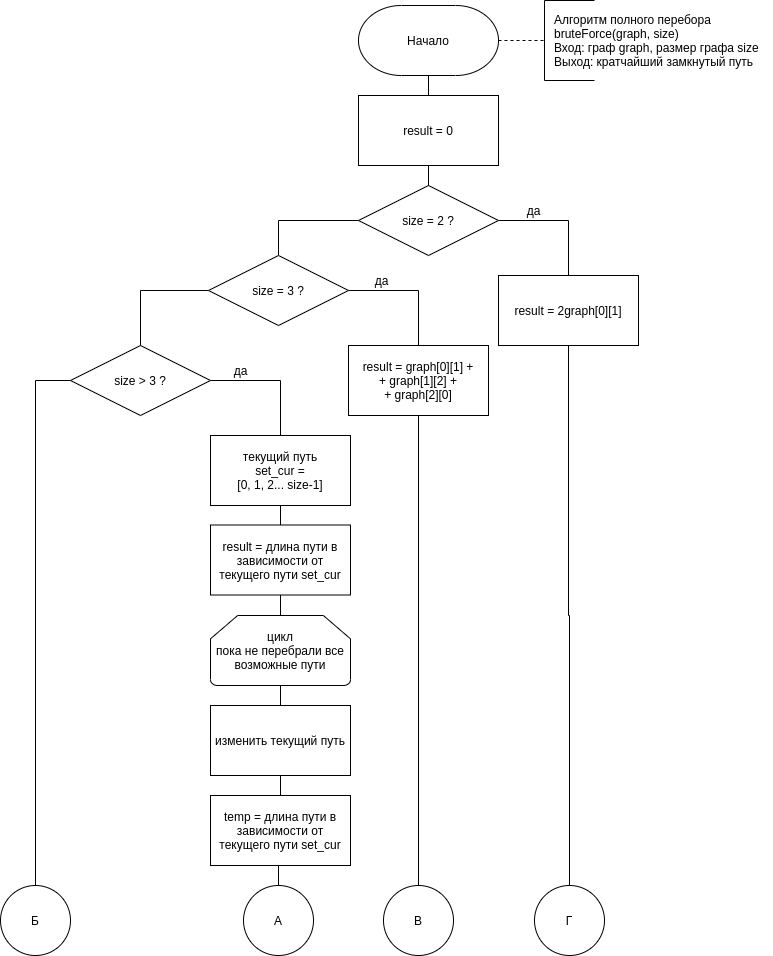
\includegraphics[scale=0.65]{brute1.png}}
		\caption*{Рисунок 2.1~--- Алгоритм полного перебора. Часть 1}
	\end{figure}
	
	\begin{figure}[H]
		\center{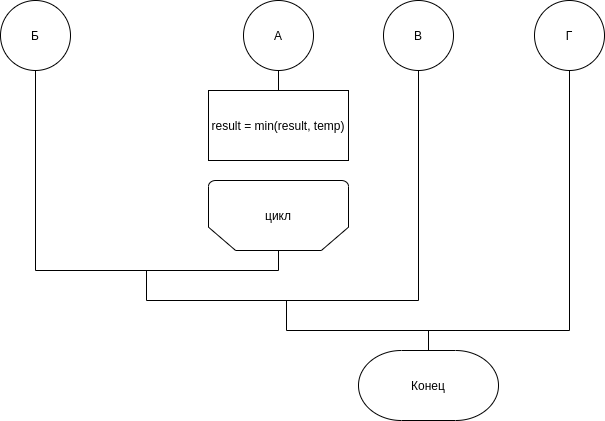
\includegraphics[scale=0.65]{brute2.png}}
		\caption*{Рисунок 2.2~--- Алгоритм полного перебора. Часть 2}
	\end{figure}
	
	\begin{figure}[H]
		\center{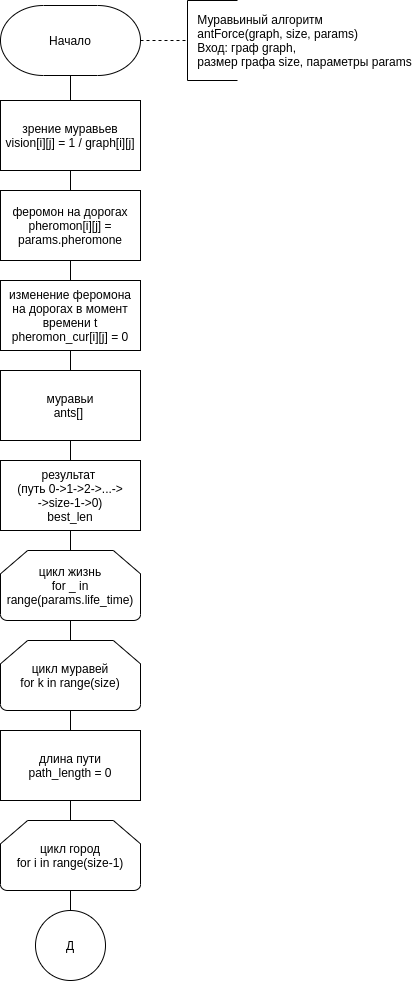
\includegraphics[scale=0.65]{ant1.png}}
		\caption*{Рисунок 2.3~--- Муравьиный алгоритм. Часть 1}
	\end{figure}
	
	\begin{figure}[H]
		\center{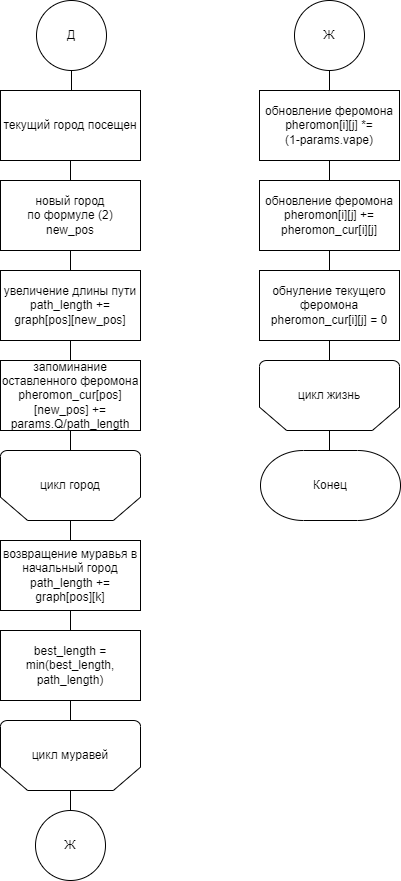
\includegraphics[scale=0.65]{ant2.png}}
		\caption*{Рисунок 2.4~--- Муравьиный алгоритм. Часть 2}
	\end{figure}
	
	\section*{2.2 Типы и структуры данных}
	\addcontentsline{toc}{section}{2.2 Типы и структуры данных}
	
	Для хранения графа используется квадратная матрица размером $n \times n$, где $n$~--- количество городов. Тип матрицы~--- целочисленная. Несмотря на то, что достаточно было бы использования верхнетреугольной или нижнетреугольной матрицы, используется полная для удобства доступа к любой длине пути.
	
	При реализации муравьиного алгоритма следует объединить входящие параметры алгоритма в отдельную структуру для минимизации количества явных передаваемых параметров в функцию, реализующую муравьиный алгоритм. Так, структура \verb|Params| содержит такие поля: $\alpha$, $\beta$, длина оптимального пути, коэффициент испарения феромона, начальное значение феромона, длина жизни колонии муравьев.
	
	Также использование структуры \verb|Ant| позволит повысить читаемость исходного кода и уменьшит количество ошибок, связанных со списком городов, которые остается посетить каждому муравью. В этой структуре выделены следующие поля: текущая позиция, список непосещенных городов~--- массив типа \verb|bool|.
	
	\section*{2.3 Способ тестирования}
	\addcontentsline{toc}{section}{2.3 Способ тестирования}
	
	Создаваемое программное обеспечение будет протестировано методом \verb|черного ящика|. Для тестирования были выделены следующие классы эквивалентности.
	\begin{enumerate}
		\item Неверный выбор режима работы программы~--- пустой ввод, нецифровой символ или вещественное число.
		\item Верный выбор режима работы программы~--- цифра из диапазона $[1..4]$ или целое число, выходящее за пределы указанного диапазона.
		\item Неверный ввод размера исходного графа~--- пустой ввод, нецифровой символ, целое неположительное число, единица или вещественное число.
		\item Верный ввод размера исходного графа~--- целое положительное число, большее единицы.
		\item Неверный ввод длины пути между городами~--- пустой ввод, нецифровой символ, целое неположительное или вещественное число.
		\item Верный ввод длины пути между городами~--- целое положительное число.
	\end{enumerate}

	\section*{2.4 Тестовые данные}
	\addcontentsline{toc}{section}{2.4 Тестовые данные}
	
	В таблицах 2.1 -- 2.3 представлены тестовые данные.
	
	\begin{table} [H]
		\caption*{Таблица 2.1~--- Функциональные тесты выбора режима работы программы}
		\begin{tabular}[l]{|c c c|}
			\hline
			Номер тестового случая & Ввод & Ожидаемый результат  \\
			
			1 & \verb|_|\tablefootnote[1]{Пустой ввод} & Неверный ввод \\\hline 
			
			2 & $\alpha$ & Неверный ввод \\\hline
			
			3 & 3.14 & Неверный ввод \\\hline
			
			4 & 1 & Введите размер графа \\\hline 
			
			5 & 2 & Введите размер графа \\\hline
			
			6 & 3 & Таблица замеров времени \\\hline
			
			7 & 4 & Выход \\\hline
			
			8 & 4 & $.$\tablefootnote[2]{Конец работы программы} \\\hline
		\end{tabular}
	\end{table}
	
	\begin{table} [H]
		\caption*{Таблица 2.2~--- Функциональные тесты ввода размера исходного графа}
		\begin{tabular}[l]{|c c c|}
			\hline
			Номер тестового случая & Ввод & Ожидаемый результат  \\
			
			1 & $\verb|_|^1$ & Неверный ввод \\\hline 
			
			2 & $\alpha$ & Неверный ввод \\\hline 
			
			3 & -3 & Неверный ввод \\\hline 
			
			4 & 1 & Неверный ввод \\\hline
			
			5 & 3.14 & Неверный ввод \\\hline
			
			6 & 2 & Введите длины путей \\\hline
		\end{tabular}
	\end{table}
	
	\begin{table} [H]
		\caption*{Таблица 2.3~--- Функциональные тесты ввода длин путей между городами}
		\begin{tabular}[l]{|c c c|}
			\hline
			Номер тестового случая & Ввод & Ожидаемый результат  \\
			
			1 & $\verb|_|^1$ & Неверный ввод \\\hline 
			
			2 & $\alpha$ & Неверный ввод \\\hline 
			
			3 & 2.2 & Неверный ввод \\\hline
			
			4 & 0 & Неверный ввод \\\hline
			
			5 & 4 & $...$\tablefootnote[3]{Ожидание ввода следующего элемента} \\\hline 
		\end{tabular}
	\end{table}
	
	\section*{2.5 Структура программного обеспечения}
	\addcontentsline{toc}{section}{2.5 Структура программного обеспечения}
	
	Программное обеспечение разработано с использованием объектно-\newlineориентированного подхода. Программа содержит функции, отвечающие за решение задачи коммивояжера. Функция \verb|bruteForce| решает данную задачу методом полного перебора всех возможных замкнутых путей. Она принимает на вход исходный граф и его размер. Функция \verb|antForce| решает задачу коммивояжера с помощью муравьиного алгоритма. Она помимо исходного графа и его размера принимает на вход все параметры, необходимые для реализации алгоритма. Обе функции возвращают целое число~--- длину кратчайшего пути, при котором будут посещены все города и конечной точкой будет начальный город~--- ответ к задаче коммивояжера.
	
	\section*{2.6 Вывод по конструкторской части}
	\addcontentsline{toc}{section}{2.6 Вывод по конструкторской части}
	
	В данном разделе были разработаны схемы алгоритмов для решения задачи коммивояжера: алгоритма полного перебора и муравьиного алгоритма, а также подготовлены тестовые данные для программного обеспечения. 
	
	\chapter*{3 Технологическая часть}
	\addcontentsline{toc}{chapter}{3 Технологическая часть}
	
	В данном разделе приведены средства реализации и листинги кода, а также перечислены требования к разрабатываемому программному обеспечению.
	
	\section*{3.1 Требования к ПО}
	\addcontentsline{toc}{section}{3.1 Требования к ПО}
	
	К программе предъявляется ряд требований:
	
	\begin{itemize}
		\item требования ко вводу
		\begin{itemize}
			\item должен быть выбран режим работы программы (целое число в диапазоне $[1..4]$);
			\item должны быть введены следующие значения: размерность графа (целое число, большее 1), длины путей между городами (натуральные числа), при необходимости: параметры $\alpha$, $p$, начальное количество феромона на ребрах графа (вещественные числа в диапазоне $[0, 1]$), параметр $t_{max}$~--- продолжительность жизни колонии муравьев (натуральное число).
		\end{itemize}
		\item требования к выводу
		\begin{itemize}
			\item найденный кратчайший путь;
			\item таблица времен работы и точности реализаций алгоритмов (точность алгоритма грубой силы эталонна) на случайных значениях.
		\end{itemize}
		\item ограничения работы программы
		\begin{itemize}
			\item при вводе режима работы программы, выходящего за пределы указанного диапазона, программа сообщает об ошибке ввода режима работы.
		\end{itemize}
		\item функциональные требования к программному обеспечению
		\begin{itemize}
			\item при запуске программа должна выводить меню с возможными режимами работы;
			\item программа должна решать задачу коммивояжера одним из двух вышеуказанных алгоритмов;
			\item в исследовательском режиме программа должна замерять время работы реализаций обоих алгоритмов, а также оценивать точность решения задачи коммивояжера муравьиным алгоритмом при случайных длинах путей между городами.
		\end{itemize}
	\end{itemize}
	
	\section*{3.2 Средства реализации}
	\addcontentsline{toc}{section}{3.2 Средства реализации}
	
	Для реализации ПО был выбран язык программирования \verb|Python| [1]. Это обусловлено знанием возможностей языка, что обеспечит высокую скорость написания программы без потери ее качества. 
	
	В качестве среды разработки была выбрана \verb|Visual Studio Code| [3]. Достаточный опыт работы в этой среде, удобства написания кода и его автодополнения стали ключевыми при выборе.
	
	\section*{3.3 Реализация алгоритмов}
	\addcontentsline{toc}{section}{3.3 Реализация алгоритмов}
	
	В листингах 3.1 -- 3.2 приведены реализации алгоритмов, использовавшихся в программном обеспечении.

	\begin{lstlisting}[title=Листинг 3.1~--- Алгоритм полного перебора]
def bruteForce(graph, size):
	result = 0
	if size == 2:
		result = 2*graph[0][1]
	elif size == 3:
		result = graph[0][1] + graph[0][2] + graph[1][2]
	elif size > 3:
		set_cur = [i for i in range(size)]
		result = lenBySet(graph, set_cur, size)
		while nextSet(set_cur, size):
			temp = lenBySet(graph, set_cur, size)
			if temp < result:
				result = temp
	return result
	\end{lstlisting}
	\newpage
	\begin{lstlisting}[title=Листинг 3.2~--- Муравьиный алгоритм]
def antForce(graph, size, params):
	vision = []
	pheromon = []
	pheromon_cur = []
	ants = []
	best_len = graph[size-1][0]
	for i in range(size):
		if i != size-1:
			best_len += graph[i][i+1]
		ants.append(Ant(i, size))
	vision.append(size*[0])
	pheromon.append(size*[params.pheromone])
	pheromon_cur.append(size*[0.0])
	for j in range(size):
		if i != j:
			vision[i][j] = 1/graph[i][j]
	for _ in range(params.life_time):
		for k in range(size):
			path_length = 0
			for i in range(size-1):
				ants[k].to_visit[ants[k].position] = 0
				probs = size*[0]
				for j in range(size):
					if not ants[k].to_visit[j]:
						probs[j] = [0, j]
					else:
						temp = 0.0
						for z in range(size):
							if ants[k].to_visit[z]:
								temp += pow(pheromon[ants[k].position][z], params.alpha)*\
										pow(vision[ants[k].position][z], params.beta)
	\end{lstlisting}
	\newpage
	\begin{lstlisting}[firstnumber=32]
						temp = pow(pheromon[ants[k].position][j], params.alpha)*\
							pow(vision[ants[k].position][j], params.beta)/temp
						probs[j] = [temp, j]
				probs.sort(key=lambda x:x[0])
				summ = 0.0
				for j in range(size):
					if probs[j][0]:
						temp = summ
						summ += probs[j][0]
						probs[j][0] += temp
				new_pos = newPos(probs, size)
				path_length += graph[ants[k].position][new_pos]
				pheromon_cur[ants[k].position][new_pos] += params.opt_len/path_length
				pheromon_cur[new_pos][ants[k].position] += params.opt_len/path_length
				ants[k].position = new_pos
			path_length += graph[ants[k].position][k]
			pheromon_cur[ants[k].position][k] += params.opt_len/path_length
			pheromon_cur[k][ants[k].position] += params.opt_len/path_length
			ants[k].position = k
			for j in range(size):
				ants[k].to_visit[j] = 1
			if best_len > path_length:
				best_len = path_length
		for i in range(size):
			for j in range(size):
				if i < j:
					pheromon[i][j] = (1-params.vape)*pheromon[i][j] + pheromon_cur[i][j]
					pheromon[j][i] = pheromon[i][j]
					pheromon_cur[i][j] = 0.0
					pheromon_cur[j][i] = 0.0
return best_len
	\end{lstlisting}
	
	\section*{3.4 Пример работы программы}
	\addcontentsline{toc}{section}{3.4 Пример работы программы}
	
	На рисунке 3.1 приведен пример работы программы.
	
	\begin{figure}[H]
		\center{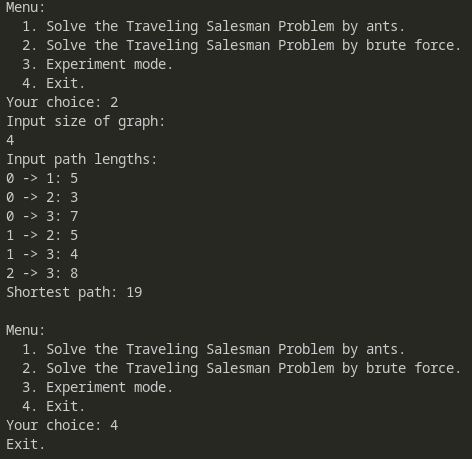
\includegraphics[scale=0.72]{example.PNG}}
		\caption*{Рисунок 3.1~--- Пример работы программы}
	\end{figure}
	
	\section*{3.5 Вывод по технологической части}
	\addcontentsline{toc}{section}{3.5 Вывод по технологической части}
	
	В данном разделе были описаны средства реализации, представлены требования к ПО и реализованы алгоритмы для решения задачи коммивояжера: алгоритм полного перебора и муравьиный алгоритм.
	
	\chapter*{4 Исследовательская часть}
	\addcontentsline{toc}{chapter}{4 Исследовательская часть}
	
	В этом разделе будет исследовано быстродействие разработанных реализаций алгоритмов и точность муравьиного алгоритма в зависимости от его входных параметров.
	
	\section*{4.1 Технические характеристики}
	\addcontentsline{toc}{section}{4.1 Технические характеристики}
	
	Ниже приведены технические характеристики устройства, на котором было проведено тестирование ПО:
	
	\begin{itemize}
		\item операционная система Windows 10 64-разрядная;
		\item оперативная память 16 ГБ;
		\item процессор Intel(R) Core(TM) i5-4690 @ 3.50ГГц.
	\end{itemize}
	
	\section*{4.2 Время выполнения реализаций алгоритмов}
	\addcontentsline{toc}{section}{4.2 Время выполнения реализаций алгоритмов}
	
	Время выполнения реализаций алгоритмов замерялось с помощью специальной функции \verb|process_time()| [2] из модуля \verb|time|, которая возвращает значение в долях секунды процессорного времени текущего процесса. Контрольная точка возвращаемого значения не определена, поэтому допустима только разница между результатами последовательных вызовов.
	
	В таблицах 4.1 и 4.2 приведены результаты замеров. В первой приведены результаты замеров при относительно одинаковых возможных длинах путей (от 10 до 50), во второй же длины путей между городами могут различаться значительно (от 10 до 500). Точностью в таблице названо число совпадений результатов работы муравьиного алгоритма и алгоритма полного перебора (из пяти итераций).
	
	\begin{table} [H]
		\caption*{Таблица 4.1~--- Время работы реализаций алгоритмов при длинах путей от 10 до 50}
		\begin{tabular}[l]{|c c c c c c c|}
			\hline
			\text{Размер} & \text{Длина жизни} & $\alpha$ & $\beta$ & \text{Точность} & \text{Время полн. перебора} & \text{Время мурав.} \\\hline
			
			3 & 10 & 0.0 & 1.0 & 5 & 0.00000219 & 0.00078882 \\
			
			3 & 10 & 0.1 & 0.9 & 5 & 0.00000084 & 0.00041421 \\
			
			3 & 10 & 0.2 & 0.8 & 5 & 0.00000034 & 0.00018570 \\
			
			3 & 10 & 0.3 & 0.7 & 5 & 0.00000035 & 0.00018318 \\
			
			3 & 10 & 0.4 & 0.6 & 5 & 0.00000033 & 0.00018223 \\
			
			3 & 10 & 0.5 & 0.5 & 5 & 0.00000034 & 0.00018198 \\
			
			3 & 10 & 0.6 & 0.4 & 5 & 0.00000037 & 0.00019560 \\
			
			3 & 10 & 0.7 & 0.3 & 5 & 0.00000036 & 0.00018212 \\
			
			3 & 10 & 0.8 & 0.2 & 5 & 0.00000036 & 0.00018297 \\
			
			3 & 10 & 0.9 & 0.1 & 5 & 0.00000033 & 0.00018294 \\
			
			3 & 10 & 1.0 & 0.0 & 5 & 0.00000032 & 0.00018285 \\
			
			3 & 50 & 0.0 & 1.0 & 5 & 0.00000033 & 0.00085964 \\
			
			3 & 50 & 0.1 & 0.9 & 5 & 0.00000033 & 0.00088145 \\
			
			3 & 50 & 0.2 & 0.8 & 5 & 0.00000033 & 0.00087717 \\
			
			3 & 50 & 0.3 & 0.7 & 5 & 0.00000035 & 0.00087489 \\
			
			3 & 50 & 0.4 & 0.6 & 5 & 0.00000033 & 0.00088073 \\
			
			3 & 50 & 0.5 & 0.5 & 5 & 0.00000032 & 0.00087492 \\
			
			3 & 50 & 0.6 & 0.4 & 5 & 0.00000036 & 0.00094207 \\
			
			3 & 50 & 0.7 & 0.3 & 5 & 0.00000034 & 0.00089784 \\
			
			3 & 50 & 0.8 & 0.2 & 5 & 0.00000036 & 0.00088677 \\
			
			3 & 50 & 0.9 & 0.1 & 5 & 0.00000034 & 0.00088047 \\
			
			3 & 50 & 1.0 & 0.0 & 5 & 0.00000035 & 0.00087933 \\
			
			3 & 100 & 0.0 & 1.0 & 5 & 0.00000035 & 0.00170278 \\
			
			3 & 100 & 0.1 & 0.9 & 5 & 0.00000037 & 0.00177776 \\
			
			3 & 100 & 0.2 & 0.8 & 5 & 0.00000035 & 0.00179710 \\
			
			3 & 100 & 0.3 & 0.7 & 5 & 0.00000035 & 0.00178699 \\
			
			3 & 100 & 0.4 & 0.6 & 5 & 0.00000036 & 0.00178131 \\
			
			3 & 100 & 0.5 & 0.5 & 5 & 0.00000036 & 0.00179008 \\
			
			3 & 100 & 0.6 & 0.4 & 5 & 0.00000035 & 0.00179600 \\
			
			3 & 100 & 0.7 & 0.3 & 5 & 0.00000036 & 0.00182403 \\
			
			3 & 100 & 0.8 & 0.2 & 5 & 0.00000036 & 0.00179437 \\
			
			3 & 100 & 0.9 & 0.1 & 5 & 0.00000034 & 0.00179425 \\
			
			3 & 100 & 1.0 & 0.0 & 5 & 0.00000065 & 0.00179299 \\\hline
		\end{tabular}
	\end{table}
	
	\begin{table} [H]
		\caption*{Таблица 4.1 (продолж.)}
		\begin{tabular}[l]{|c c c c c c c|}
			\hline
			\text{Размер} & \text{Длина жизни} & $\alpha$ & $\beta$ & \text{Точность} & \text{Время полн. перебора} & \text{Время мурав.} \\\hline
			5 & 10 & 0.0 & 1.0 & 5 & 0.00008234 & 0.00097245 \\
			
			5 & 10 & 0.1 & 0.9 & 5 & 0.00008125 & 0.00099766 \\
			
			5 & 10 & 0.2 & 0.8 & 5 & 0.00008129 & 0.00103464 \\
			
			5 & 10 & 0.3 & 0.7 & 5 & 0.00008028 & 0.00099031 \\
			
			5 & 10 & 0.4 & 0.6 & 5 & 0.00008114 & 0.00099809 \\
			
			5 & 10 & 0.5 & 0.5 & 5 & 0.00008147 & 0.00101160 \\
			
			5 & 10 & 0.6 & 0.4 & 5 & 0.00008073 & 0.00100438 \\
			
			5 & 10 & 0.7 & 0.3 & 5 & 0.00007975 & 0.00100827 \\
			
			5 & 10 & 0.8 & 0.2 & 4 & 0.00008039 & 0.00100578 \\
			
			5 & 10 & 0.9 & 0.1 & 5 & 0.00007988 & 0.00100109 \\
			
			5 & 10 & 1.0 & 0.0 & 5 & 0.00008171 & 0.00101838 \\
			
			5 & 50 & 0.0 & 1.0 & 5 & 0.00008018 & 0.00479159 \\
			
			5 & 50 & 0.1 & 0.9 & 5 & 0.00008126 & 0.00500221 \\
			
			5 & 50 & 0.2 & 0.8 & 5 & 0.00008132 & 0.00501788 \\
			
			5 & 50 & 0.3 & 0.7 & 5 & 0.00008105 & 0.00502501 \\
			
			5 & 50 & 0.4 & 0.6 & 5 & 0.00008084 & 0.00498023 \\
			
			5 & 50 & 0.5 & 0.5 & 5 & 0.00008028 & 0.00501089 \\
			
			5 & 50 & 0.6 & 0.4 & 5 & 0.00008124 & 0.00504253 \\
			
			5 & 50 & 0.7 & 0.3 & 5 & 0.00008204 & 0.00501831 \\
			
			5 & 50 & 0.8 & 0.2 & 5 & 0.00008240 & 0.00501918 \\
			
			5 & 50 & 0.9 & 0.1 & 5 & 0.00008108 & 0.00503401 \\
			
			5 & 50 & 1.0 & 0.0 & 5 & 0.00008176 & 0.00504283 \\
			
			5 & 100 & 0.0 & 1.0 & 5 & 0.00008248 & 0.00963954 \\
			
			5 & 100 & 0.1 & 0.9 & 5 & 0.00008121 & 0.01006820 \\
			
			5 & 100 & 0.2 & 0.8 & 5 & 0.00008212 & 0.01005573 \\
			
			5 & 100 & 0.3 & 0.7 & 5 & 0.00008191 & 0.01000944 \\
			
			5 & 100 & 0.4 & 0.6 & 5 & 0.00008123 & 0.01008802 \\
			
			5 & 100 & 0.5 & 0.5 & 5 & 0.00008327 & 0.01011338 \\
			
			5 & 100 & 0.6 & 0.4 & 5 & 0.00008212 & 0.01011456 \\
			
			5 & 100 & 0.7 & 0.3 & 5 & 0.00008270 & 0.01012282 \\
			
			5 & 100 & 0.8 & 0.2 & 5 & 0.00008134 & 0.01010857 \\
			
			5 & 100 & 0.9 & 0.1 & 5 & 0.00008162 & 0.01007508 \\
			
			5 & 100 & 1.0 & 0.0 & 5 & 0.00008352 & 0.01013730 \\\hline
		\end{tabular}
	\end{table}
	
	\begin{table} [H]
		\caption*{Таблица 4.1 (продолж.)}
		\begin{tabular}[l]{|c c c c c c c|}
			\hline
			\text{Размер} & \text{Длина жизни} & $\alpha$ & $\beta$ & \text{Точность} & \text{Время полн. перебора} & \text{Время мурав.} \\\hline
			
			7 & 10 & 0.0 & 1.0 & 2 & 0.00390088 & 0.00317735 \\
			
			7 & 10 & 0.1 & 0.9 & 3 & 0.00391717 & 0.00334396 \\
			
			7 & 10 & 0.2 & 0.8 & 3 & 0.00394429 & 0.00329568 \\
			
			7 & 10 & 0.3 & 0.7 & 5 & 0.00391351 & 0.00331139 \\
			
			7 & 10 & 0.4 & 0.6 & 4 & 0.00392883 & 0.00333498 \\
			
			7 & 10 & 0.5 & 0.5 & 3 & 0.00391856 & 0.00332484 \\
			
			7 & 10 & 0.6 & 0.4 & 5 & 0.00390492 & 0.00332260 \\
			
			7 & 10 & 0.7 & 0.3 & 4 & 0.00387885 & 0.00331713 \\
			
			7 & 10 & 0.8 & 0.2 & 2 & 0.00390997 & 0.00330329 \\
			
			7 & 10 & 0.9 & 0.1 & 1 & 0.00387674 & 0.00330903 \\
			
			7 & 10 & 1.0 & 0.0 & 3 & 0.00396468 & 0.00332733 \\
			
			7 & 50 & 0.0 & 1.0 & 5 & 0.00389941 & 0.01569061 \\
			
			7 & 50 & 0.1 & 0.9 & 5 & 0.00389956 & 0.01639940 \\
			
			7 & 50 & 0.2 & 0.8 & 5 & 0.00386870 & 0.01652652 \\
			
			7 & 50 & 0.3 & 0.7 & 5 & 0.00390567 & 0.01642507 \\
			
			7 & 50 & 0.4 & 0.6 & 5 & 0.00397815 & 0.01673648 \\
			
			7 & 50 & 0.5 & 0.5 & 5 & 0.00391534 & 0.01657062 \\
			
			7 & 50 & 0.6 & 0.4 & 5 & 0.00391928 & 0.01666064 \\
			
			7 & 50 & 0.7 & 0.3 & 5 & 0.00396597 & 0.01659956 \\
			
			7 & 50 & 0.8 & 0.2 & 5 & 0.00394941 & 0.01667409 \\
			
			7 & 50 & 0.9 & 0.1 & 5 & 0.00394745 & 0.01664485 \\
			
			7 & 50 & 1.0 & 0.0 & 5 & 0.00391879 & 0.01668132 \\
			
			7 & 100 & 0.0 & 1.0 & 5 & 0.00394480 & 0.03162796 \\
			
			7 & 100 & 0.1 & 0.9 & 5 & 0.00396030 & 0.03331885 \\
			
			7 & 100 & 0.2 & 0.8 & 5 & 0.00393197 & 0.03292885 \\
			
			7 & 100 & 0.3 & 0.7 & 5 & 0.00389110 & 0.03308667 \\
			
			7 & 100 & 0.4 & 0.6 & 5 & 0.00394055 & 0.03314562 \\
			
			7 & 100 & 0.5 & 0.5 & 5 & 0.00402526 & 0.03326070 \\
			
			7 & 100 & 0.6 & 0.4 & 5 & 0.00399044 & 0.03315323 \\
			
			7 & 100 & 0.7 & 0.3 & 5 & 0.00401980 & 0.03340191 \\
			
			7 & 100 & 0.8 & 0.2 & 5 & 0.00393757 & 0.03330504 \\
			
			7 & 100 & 0.9 & 0.1 & 5 & 0.00392084 & 0.03315402 \\
			
			7 & 100 & 1.0 & 0.0 & 4 & 0.00393564 & 0.03345400 \\\hline
		\end{tabular}
	\end{table}
	
	\begin{table} [H]
		\caption*{Таблица 4.1 (продолж.)}
		\begin{tabular}[l]{|c c c c c c c|}
			\hline
			\text{Размер} & \text{Длина жизни} & $\alpha$ & $\beta$ & \text{Точность} & \text{Время полн. перебора} & \text{Время мурав.} \\\hline
			
			9 & 10 & 0.0 & 1.0 & 0 & 0.41131790 & 0.00991216 \\
			
			9 & 10 & 0.1 & 0.9 & 1 & 0.37120794 & 0.00929422 \\
			
			9 & 10 & 0.2 & 0.8 & 0 & 0.35666487 & 0.00884292 \\
			
			9 & 10 & 0.3 & 0.7 & 2 & 0.32776446 & 0.00821195 \\
			
			9 & 10 & 0.4 & 0.6 & 1 & 0.33273496 & 0.00906158 \\
			
			9 & 10 & 0.5 & 0.5 & 1 & 0.39692422 & 0.00898752 \\
			
			9 & 10 & 0.6 & 0.4 & 2 & 0.32793279 & 0.00821731 \\
			
			9 & 10 & 0.7 & 0.3 & 0 & 0.39141998 & 0.00988386 \\
			
			9 & 10 & 0.8 & 0.2 & 0 & 0.32636173 & 0.00827970 \\
			
			9 & 10 & 0.9 & 0.1 & 0 & 0.32877880 & 0.00828145 \\
			
			9 & 10 & 1.0 & 0.0 & 1 & 0.32997707 & 0.00828740 \\
			
			9 & 50 & 0.0 & 1.0 & 1 & 0.32823027 & 0.03906523 \\
			
			9 & 50 & 0.1 & 0.9 & 1 & 0.32877006 & 0.04125859 \\
			
			9 & 50 & 0.2 & 0.8 & 3 & 0.32958525 & 0.04121013 \\
			
			9 & 50 & 0.3 & 0.7 & 4 & 0.32797867 & 0.04158168 \\
			
			9 & 50 & 0.4 & 0.6 & 3 & 0.32962953 & 0.04118422 \\
			
			9 & 50 & 0.5 & 0.5 & 3 & 0.32817190 & 0.04154504 \\
			
			9 & 50 & 0.6 & 0.4 & 3 & 0.35727065 & 0.04555401 \\
			
			9 & 50 & 0.7 & 0.3 & 3 & 0.55569646 & 0.05950507 \\
			
			9 & 50 & 0.8 & 0.2 & 5 & 0.57243198 & 0.06031459 \\
			
			9 & 50 & 0.9 & 0.1 & 5 & 0.55894089 & 0.05924416 \\
			
			9 & 50 & 1.0 & 0.0 & 2 & 0.56761876 & 0.05973323 \\
			
			9 & 100 & 0.0 & 1.0 & 0 & 0.56204300 & 0.11373902 \\
			
			9 & 100 & 0.1 & 0.9 & 3 & 0.55952135 & 0.11841433 \\
			
			9 & 100 & 0.2 & 0.8 & 2 & 0.57111101 & 0.12085845 \\
			
			9 & 100 & 0.3 & 0.7 & 3 & 0.56669370 & 0.12064041 \\
			
			9 & 100 & 0.4 & 0.6 & 5 & 0.56082930 & 0.11856957 \\
			
			9 & 100 & 0.5 & 0.5 & 5 & 0.56987188 & 0.11912484 \\
			
			9 & 100 & 0.6 & 0.4 & 3 & 0.56953865 & 0.11965193 \\
			
			9 & 100 & 0.7 & 0.3 & 5 & 0.56507396 & 0.11958399 \\
			
			9 & 100 & 0.8 & 0.2 & 5 & 0.56631942 & 0.12077165 \\
			
			9 & 100 & 0.9 & 0.1 & 5 & 0.56608504 & 0.11889582 \\
			
			9 & 100 & 1.0 & 0.0 & 5 & 0.55832422 & 0.11897110 \\\hline
		\end{tabular}
	\end{table}
	
	\begin{table} [H]
		\caption*{Таблица 4.2~--- Время работы реализаций алгоритмов при длинах путей от 10 до 500}
		\begin{tabular}[l]{|c c c c c c c|}
			\hline
			\text{Размер} & \text{Длина жизни} & $\alpha$ & $\beta$ & \text{Точность} & \text{Время полн. перебора} & \text{Время мурав.} \\\hline
			
			3 & 10 & 0.0 & 1.0 & 5 & 0.00000051 & 0.00027483 \\
			
			3 & 10 & 0.1 & 0.9 & 5 & 0.00000045 & 0.00026964 \\
			
			3 & 10 & 0.2 & 0.8 & 5 & 0.00000045 & 0.00027447 \\
			
			3 & 10 & 0.3 & 0.7 & 5 & 0.00000046 & 0.00027675 \\
			
			3 & 10 & 0.4 & 0.6 & 5 & 0.00000045 & 0.00027581 \\
			
			3 & 10 & 0.5 & 0.5 & 5 & 0.00000046 & 0.00027470 \\
			
			3 & 10 & 0.6 & 0.4 & 5 & 0.00000046 & 0.00027806 \\
			
			3 & 10 & 0.7 & 0.3 & 5 & 0.00000043 & 0.00027488 \\
			
			3 & 10 & 0.8 & 0.2 & 5 & 0.00000045 & 0.00027612 \\
			
			3 & 10 & 0.9 & 0.1 & 5 & 0.00000045 & 0.00027632 \\
			
			3 & 10 & 1.0 & 0.0 & 5 & 0.00000045 & 0.00027627 \\
			
			3 & 50 & 0.0 & 1.0 & 5 & 0.00000044 & 0.00130708 \\
			
			3 & 50 & 0.1 & 0.9 & 5 & 0.00000044 & 0.00133097 \\
			
			3 & 50 & 0.2 & 0.8 & 5 & 0.00000043 & 0.00133850 \\
			
			3 & 50 & 0.3 & 0.7 & 5 & 0.00000044 & 0.00133814 \\
			
			3 & 50 & 0.4 & 0.6 & 5 & 0.00000046 & 0.00133159 \\
			
			3 & 50 & 0.5 & 0.5 & 5 & 0.00000043 & 0.00132636 \\
			
			3 & 50 & 0.6 & 0.4 & 5 & 0.00000044 & 0.00133234 \\
			
			3 & 50 & 0.7 & 0.3 & 5 & 0.00000044 & 0.00132780 \\
			
			3 & 50 & 0.8 & 0.2 & 5 & 0.00000046 & 0.00133007 \\
			
			3 & 50 & 0.9 & 0.1 & 5 & 0.00000044 & 0.00132219 \\
			
			3 & 50 & 1.0 & 0.0 & 5 & 0.00000046 & 0.00136712 \\
			
			3 & 100 & 0.0 & 1.0 & 5 & 0.00000043 & 0.00258292 \\
			
			3 & 100 & 0.1 & 0.9 & 5 & 0.00000045 & 0.00264400 \\
			
			3 & 100 & 0.2 & 0.8 & 5 & 0.00000048 & 0.00266488 \\
			
			3 & 100 & 0.3 & 0.7 & 5 & 0.00000047 & 0.00265973 \\
			
			3 & 100 & 0.4 & 0.6 & 5 & 0.00000046 & 0.00268160 \\
			
			3 & 100 & 0.5 & 0.5 & 5 & 0.00000044 & 0.00265839 \\
			
			3 & 100 & 0.6 & 0.4 & 5 & 0.00000045 & 0.00264781 \\
			
			3 & 100 & 0.7 & 0.3 & 5 & 0.00000045 & 0.00265933 \\
			
			3 & 100 & 0.8 & 0.2 & 5 & 0.00000044 & 0.00268129 \\
			
			3 & 100 & 0.9 & 0.1 & 5 & 0.00000045 & 0.00265221 \\
			
			3 & 100 & 1.0 & 0.0 & 5 & 0.00000044 & 0.00266374 \\\hline
		\end{tabular}
	\end{table}
	
	\begin{table} [H]
		\caption*{Таблица 4.2 (продолж.)}
		\begin{tabular}[l]{|c c c c c c c|}
			\hline
			\text{Размер} & \text{Длина жизни} & $\alpha$ & $\beta$ & \text{Точность} & \text{Время полн. перебора} & \text{Время мурав.} \\\hline
			
			5 & 10 & 0.0 & 1.0 & 5 & 0.00015329 & 0.00150426 \\
			
			5 & 10 & 0.1 & 0.9 & 5 & 0.00015133 & 0.00156364 \\
			
			5 & 10 & 0.2 & 0.8 & 5 & 0.00015108 & 0.00155528 \\
			
			5 & 10 & 0.3 & 0.7 & 5 & 0.00015012 & 0.00155513 \\
			
			5 & 10 & 0.4 & 0.6 & 5 & 0.00015169 & 0.00156079 \\
			
			5 & 10 & 0.5 & 0.5 & 5 & 0.00014993 & 0.00155889 \\
			
			5 & 10 & 0.6 & 0.4 & 5 & 0.00015135 & 0.00155541 \\
			
			5 & 10 & 0.7 & 0.3 & 5 & 0.00015091 & 0.00155550 \\
			
			5 & 10 & 0.8 & 0.2 & 5 & 0.00015066 & 0.00155332 \\
			
			5 & 10 & 0.9 & 0.1 & 5 & 0.00015287 & 0.00156550 \\
			
			5 & 10 & 1.0 & 0.0 & 4 & 0.00014941 & 0.00156148 \\
			
			5 & 50 & 0.0 & 1.0 & 5 & 0.00015032 & 0.00742698 \\
			
			5 & 50 & 0.1 & 0.9 & 5 & 0.00015113 & 0.00771625 \\
			
			5 & 50 & 0.2 & 0.8 & 5 & 0.00015027 & 0.00769867 \\
			
			5 & 50 & 0.3 & 0.7 & 5 & 0.00015005 & 0.00766503 \\
			
			5 & 50 & 0.4 & 0.6 & 5 & 0.00015009 & 0.00772060 \\
			
			5 & 50 & 0.5 & 0.5 & 5 & 0.00014960 & 0.00761381 \\
			
			5 & 50 & 0.6 & 0.4 & 5 & 0.00014975 & 0.00757860 \\
			
			5 & 50 & 0.7 & 0.3 & 5 & 0.00015013 & 0.00759881 \\
			
			5 & 50 & 0.8 & 0.2 & 5 & 0.00014947 & 0.00756942 \\
			
			5 & 50 & 0.9 & 0.1 & 5 & 0.00014927 & 0.00755403 \\
			
			5 & 50 & 1.0 & 0.0 & 5 & 0.00014754 & 0.00755866 \\
			
			5 & 100 & 0.0 & 1.0 & 5 & 0.00014930 & 0.01451482 \\
			
			5 & 100 & 0.1 & 0.9 & 5 & 0.00014964 & 0.01520552 \\
			
			5 & 100 & 0.2 & 0.8 & 5 & 0.00014933 & 0.01519972 \\
			
			5 & 100 & 0.3 & 0.7 & 5 & 0.00015037 & 0.01498814 \\
			
			5 & 100 & 0.4 & 0.6 & 5 & 0.00014759 & 0.01491379 \\
			
			5 & 100 & 0.5 & 0.5 & 5 & 0.00014860 & 0.01493828 \\
			
			5 & 100 & 0.6 & 0.4 & 5 & 0.00015161 & 0.01502105 \\
			
			5 & 100 & 0.7 & 0.3 & 5 & 0.00015101 & 0.01514263 \\
			
			5 & 100 & 0.8 & 0.2 & 5 & 0.00015009 & 0.01503636 \\
			
			5 & 100 & 0.9 & 0.1 & 5 & 0.00014976 & 0.01520454 \\
			
			5 & 100 & 1.0 & 0.0 & 5 & 0.00014984 & 0.01527121 \\\hline
		\end{tabular}
	\end{table}
	
	\begin{table} [H]
		\caption*{Таблица 4.2 (продолж.)}
		\begin{tabular}[l]{|c c c c c c c|}
			\hline
			\text{Размер} & \text{Длина жизни} & $\alpha$ & $\beta$ & \text{Точность} & \text{Время полн. перебора} & \text{Время мурав.} \\\hline
			
			7 & 10 & 0.0 & 1.0 & 5 & 0.00722309 & 0.00477381 \\
			
			7 & 10 & 0.1 & 0.9 & 5 & 0.00722765 & 0.00500741 \\
			
			7 & 10 & 0.2 & 0.8 & 3 & 0.00725934 & 0.00499453 \\
			
			7 & 10 & 0.3 & 0.7 & 4 & 0.00711199 & 0.00491041 \\
			
			7 & 10 & 0.4 & 0.6 & 4 & 0.00708778 & 0.00490368 \\
			
			7 & 10 & 0.5 & 0.5 & 4 & 0.00700027 & 0.00488140 \\
			
			7 & 10 & 0.6 & 0.4 & 4 & 0.00710628 & 0.00477898 \\
			
			7 & 10 & 0.7 & 0.3 & 3 & 0.00709041 & 0.00467442 \\
			
			7 & 10 & 0.8 & 0.2 & 3 & 0.00705312 & 0.00468630 \\
			
			7 & 10 & 0.9 & 0.1 & 3 & 0.00712018 & 0.00469490 \\
			
			7 & 10 & 1.0 & 0.0 & 3 & 0.00708587 & 0.00469429 \\
			
			7 & 50 & 0.0 & 1.0 & 5 & 0.00702237 & 0.02299568 \\
			
			7 & 50 & 0.1 & 0.9 & 5 & 0.00711434 & 0.02337047 \\
			
			7 & 50 & 0.2 & 0.8 & 5 & 0.00709199 & 0.02344858 \\
			
			7 & 50 & 0.3 & 0.7 & 5 & 0.00717292 & 0.02344074 \\
			
			7 & 50 & 0.4 & 0.6 & 5 & 0.00719640 & 0.02379326 \\
			
			7 & 50 & 0.5 & 0.5 & 5 & 0.00731073 & 0.02404188 \\
			
			7 & 50 & 0.6 & 0.4 & 5 & 0.00724545 & 0.02376892 \\
			
			7 & 50 & 0.7 & 0.3 & 5 & 0.00722176 & 0.02374369 \\
			
			7 & 50 & 0.8 & 0.2 & 4 & 0.00723187 & 0.02382991 \\
			
			7 & 50 & 0.9 & 0.1 & 5 & 0.00724902 & 0.02378414 \\
			
			7 & 50 & 1.0 & 0.0 & 4 & 0.00708376 & 0.02333004 \\
			
			7 & 100 & 0.0 & 1.0 & 5 & 0.00713661 & 0.04638983 \\
			
			7 & 100 & 0.1 & 0.9 & 5 & 0.00721081 & 0.04732876 \\
			
			7 & 100 & 0.2 & 0.8 & 5 & 0.00723819 & 0.04756339 \\
			
			7 & 100 & 0.3 & 0.7 & 5 & 0.00717817 & 0.04731467 \\
			
			7 & 100 & 0.4 & 0.6 & 5 & 0.00717493 & 0.04675035 \\
			
			7 & 100 & 0.5 & 0.5 & 5 & 0.00691494 & 0.04506613 \\
			
			7 & 100 & 0.6 & 0.4 & 5 & 0.00696528 & 0.04511164 \\
			
			7 & 100 & 0.7 & 0.3 & 5 & 0.00686388 & 0.04536150 \\
			
			7 & 100 & 0.8 & 0.2 & 5 & 0.00692658 & 0.04580344 \\
			
			7 & 100 & 0.9 & 0.1 & 5 & 0.00694621 & 0.04601983 \\
			
			7 & 100 & 1.0 & 0.0 & 5 & 0.00691595 & 0.04633113 \\\hline
		\end{tabular}
	\end{table}
	
	\begin{table} [H]
		\caption*{Таблица 4.2 (продолж.)}
		\begin{tabular}[l]{|c c c c c c c|}
			\hline
			\text{Размер} & \text{Длина жизни} & $\alpha$ & $\beta$ & \text{Точность} & \text{Время полн. перебора} & \text{Время мурав.} \\\hline
			
			9 & 10 & 0.0 & 1.0 & 3 & 0.56953802 & 0.01126735 \\
			
			9 & 10 & 0.1 & 0.9 & 0 & 0.56461737 & 0.01137432 \\
			
			9 & 10 & 0.2 & 0.8 & 3 & 0.56095980 & 0.01142844 \\
			
			9 & 10 & 0.3 & 0.7 & 1 & 0.57596527 & 0.01151098 \\
			
			9 & 10 & 0.4 & 0.6 & 0 & 0.57362612 & 0.01137042 \\
			
			9 & 10 & 0.5 & 0.5 & 0 & 0.56511071 & 0.01132695 \\
			
			9 & 10 & 0.6 & 0.4 & 3 & 0.56856427 & 0.01151129 \\
			
			9 & 10 & 0.7 & 0.3 & 4 & 0.57450196 & 0.01150368 \\
			
			9 & 10 & 0.8 & 0.2 & 1 & 0.58161975 & 0.01151782 \\
			
			9 & 10 & 0.9 & 0.1 & 1 & 0.56220697 & 0.01135985 \\
			
			9 & 10 & 1.0 & 0.0 & 1 & 0.57084538 & 0.01147069 \\
			
			9 & 50 & 0.0 & 1.0 & 3 & 0.58971276 & 0.05691730 \\
			
			9 & 50 & 0.1 & 0.9 & 3 & 0.56066670 & 0.05605785 \\
			
			9 & 50 & 0.2 & 0.8 & 5 & 0.57000091 & 0.05695092 \\
			
			9 & 50 & 0.3 & 0.7 & 4 & 0.56561937 & 0.05670521 \\
			
			9 & 50 & 0.4 & 0.6 & 4 & 0.57164225 & 0.05692357 \\
			
			9 & 50 & 0.5 & 0.5 & 5 & 0.57182183 & 0.05719912 \\
			
			9 & 50 & 0.6 & 0.4 & 4 & 0.56485867 & 0.05670624 \\
			
			9 & 50 & 0.7 & 0.3 & 4 & 0.56994893 & 0.05726910 \\
			
			9 & 50 & 0.8 & 0.2 & 5 & 0.57125262 & 0.05707906 \\
			
			9 & 50 & 0.9 & 0.1 & 5 & 0.56632235 & 0.05630520 \\
			
			9 & 50 & 1.0 & 0.0 & 4 & 0.56707140 & 0.05631264 \\
			
			9 & 100 & 0.0 & 1.0 & 5 & 0.37119206 & 0.08174221 \\
			
			9 & 100 & 0.1 & 0.9 & 5 & 0.56988004 & 0.11301679 \\
			
			9 & 100 & 0.2 & 0.8 & 4 & 0.56630840 & 0.11419434 \\
			
			9 & 100 & 0.3 & 0.7 & 5 & 0.57213590 & 0.11406609 \\
			
			9 & 100 & 0.4 & 0.6 & 5 & 0.56611648 & 0.11420414 \\
			
			9 & 100 & 0.5 & 0.5 & 5 & 0.56483259 & 0.11411940 \\
			
			9 & 100 & 0.6 & 0.4 & 4 & 0.56650787 & 0.11278648 \\
			
			9 & 100 & 0.7 & 0.3 & 5 & 0.57804824 & 0.11418779 \\
			
			9 & 100 & 0.8 & 0.2 & 4 & 0.56481363 & 0.11366978 \\
			
			9 & 100 & 0.9 & 0.1 & 5 & 0.56938602 & 0.11386458 \\
			
			9 & 100 & 1.0 & 0.0 & 3 & 0.57131235 & 0.11474000 \\\hline
		\end{tabular}
	\end{table}
	
	\section*{4.3 Вывод по исследовательской части}
	\addcontentsline{toc}{section}{4.3 Вывод по исследовательской части}
	
	По результатам замеров можно сделать несколько выводов, каждый из которых может опираться на различные входные данные.
	
	Вне зависимости от длин путей между городами на малых размерах исходного графа алгоритм полного перебора будет давать результат лучше, поскольку не так много времени займет перебор всех возможных путей. В совокупности с эталонной точностью алгоритм полного перебора на малых размерах графа, а именно~--- до 6 городов, имеет выигрыш во времени вне зависимости от остальных параметров.
	
	Длина жизни колонии муравьев влияет на время выполнения реализации муравьиного алгоритма. Так, с увеличением времени жизни возрастает время выполнения. Поэтому лучшие времена муравьиный алгоритм показывает при наименьших временах жизни колонии. При этом малое время жизни дает низкий показатель точности при количестве городов большем 5. Можно сказать, что на больших размерах для достижения высокого показателя точности необходимо указывать достаточное время жизни колонии муравьев, при этом можно достичь эталонной точности при высокой производительности муравьиного алгоритма.
	
	Если рассматривать влияние параметров $\alpha$ и $\beta$ на точность вычислений, то можно заметить, что при малом количестве городов они не влияют на точность, муравьиный алгоритм и так вычисляет оптимальную длину пути с эталонной точностью. При количестве городов большем 5 и длинах путей от 10 до 50 самый стабильный средний результат показывает пара $\alpha = 0.4$ и $\beta = 0.6$, а при длинах путей от 10 до 500~--- $\alpha = 0.7$ и $\beta = 0.3$.
	
	
	\chapter*{Заключение}
	\addcontentsline{toc}{chapter}{Заключение}
	
	В ходе проделанной работы была достигнута поставленная цель и решены следующие задачи:
	
	\begin{itemize}
		\item изучены алгоритм полного перебора и муравьиный алгоритм для решения задачи коммивояжера;
		\item разработаны схемы этих алгоритмов;
		\item реализованы изученные алгоритмы;
		\item проведено тестирование разработанного программного обеспечения;
		\item проведен анализ скорости работы реализаций алгоритмов.
	\end{itemize}
	
	Было доказано, что при количестве городов меньшем 7 алгоритм полного перебора показывает лучшую производительность в совокуности с эталонной точностью. при больших размерностях исходного графа муравьиный алгоритм для демонстрации хорошей точности требует продолжительности жизни колонии муравьев большей 100. Несмотря на то, что увеличение этого параметра влечет увеличение времени выполнения алгоритма, он все равно будет давать лучший показатель производительности за счет того, что при таких размерностях графа в алгоритме грубой силы необходимо перебрать огромное количество возможных замкнутых путей.
	
	\chapter*{Список литературы}
	\addcontentsline{toc}{chapter}{Список литературы}
	
	[1] Python [Электронный ресурс]. Режим доступа: https://python.org/. Дата обращения: 25.12.2021.\\
	
	[2] Функция process\underline{ }time [Электронный ресурс]. Режим доступа: \newline https://docs.python.org/3/library/time.html. Дата обращения: 25.12.2021.\\
	
	[3] Visual Studio Code - Code Editing [Электронный ресурс]. Режим доступа: https://code.visualstudio.com. Дата обращения: 25.12.2021.\\
	
	[4] Задача коммивояжера [Электронный ресурс]. Режим доступа: \newline https://science.fandom.com/ru/wiki/zadacha-kommivoyazshera. \newline Дата обращения: 25.12.2021.
	
\end{document}